% This LaTeX was auto-generated from MATLAB code.
% To make changes, update the MATLAB code and export to LaTeX again.

\documentclass{article}

\usepackage[utf8]{inputenc}
\usepackage[T1]{fontenc}
\usepackage{lmodern}
\usepackage{graphicx}
\usepackage{color}
\usepackage{hyperref}
\usepackage{amsmath}
\usepackage{amsfonts}
\usepackage{epstopdf}
\usepackage[table]{xcolor}
\usepackage{matlab}

\sloppy
\epstopdfsetup{outdir=./}
\graphicspath{ {./RealMassMAtrix_images/} }

\begin{document}

\matlabtitle{Real Mass Matrix}

\begin{par}
\begin{flushleft}
Yo calulculate the real mass matrix  frist we devivided the Sparus into 8 different elements. For each element we will calculate a  real mass matrix, translate it into the center of mass of the SPARUS, and finally we will add ll the element matrices into a Total Mass matrix 
\end{flushleft}
\end{par}


\vspace{1em}
\begin{par}
\begin{flushleft}
The elements are the following: 
\end{flushleft}
\end{par}

\begin{itemize}
\setlength{\itemsep}{-1ex}
   \item{\begin{flushleft} Cilinder  \end{flushleft}}
   \item{\begin{flushleft} Top sphere \end{flushleft}}
   \item{\begin{flushleft} Bottom sphere \end{flushleft}}
   \item{\begin{flushleft} Antena \end{flushleft}}
   \item{\begin{flushleft} Thruster 1 \end{flushleft}}
   \item{\begin{flushleft} Thruster 2  \end{flushleft}}
   \item{\begin{flushleft} Sensor 1  \end{flushleft}}
   \item{\begin{flushleft} Sensor 2 \end{flushleft}}
\end{itemize}

\matlabheading{Volumes}

\begin{matlabcode}
v_cylinder = 0.0519;
v_topsphere = 0.0078;
v_bottomsphere = 0.0028;
v_antena = 0.00059;
v_thruster1 =  0.0003965;
v_thurster2 = 0.0003965;
v_sesnor1 =  0.000098;
v_sensor2 = 0.000059;
\end{matlabcode}

\begin{par}
\begin{flushleft}
Each volume was calulated using regular volumetric formulas, excpet for bottom sphere which was calulated by measurmente 5 diferent points and aporximating a function that has a similar shape than the sphere. then integrating.
\end{flushleft}
\end{par}


\vspace{1em}
\begin{par}
\begin{center}
 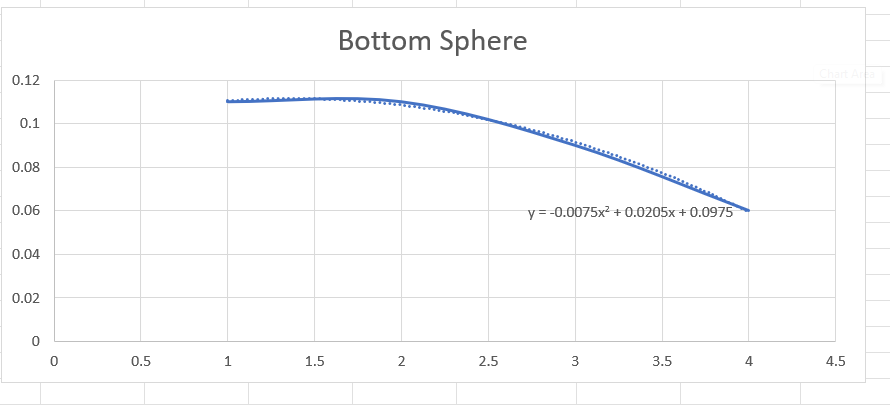
\includegraphics[width=\maxwidth{58.203712995484196em}]{image_0}
\end{center}
\end{par}

\begin{itemize}
\setlength{\itemsep}{-1ex}
   \item{\begin{flushleft} From this experiment, comparing wiht values form collegues,  we can can determine that  even though this method is more accurate the diference between integratign the curve and usign a simple shape like a sphere  is negligable (10e-3) so for future Drag and Added mass matrix  common geometry will be used for the sake of simpler calculations.  \end{flushleft}}
\end{itemize}

\begin{par}
\begin{flushleft}
We made the asumption that every part of the SPARUS has the same density. 
\end{flushleft}
\end{par}

\begin{matlabcode}
total_volume = v_cylinder+v_sensor2+v_sesnor1+v_thurster2+v_thruster1+v_bottomsphere+v_topsphere+v_antena
\end{matlabcode}
\begin{matlaboutput}
total_volume = 0.0640
\end{matlaboutput}

\begin{par}
\begin{flushleft}
From the total volume and the weight we can calulate the denisty to finally compute the mass of each element 
\end{flushleft}
\end{par}


\vspace{1em}
\matlabheading{Masses}

\begin{matlabcode}
m_SPARUS = 52;
density_SPARUS = m_SPARUS/total_volume 
\end{matlabcode}
\begin{matlaboutput}
density_SPARUS = 811.9925
\end{matlaboutput}
\begin{matlabcode}

m_cylinder = v_cylinder*density_SPARUS
\end{matlabcode}
\begin{matlaboutput}
m_cylinder = 42.1424
\end{matlaboutput}
\begin{matlabcode}
m_topsphere = v_topsphere*density_SPARUS
\end{matlabcode}
\begin{matlaboutput}
m_topsphere = 6.3335
\end{matlaboutput}
\begin{matlabcode}
m_bottomsphere = v_bottomsphere*density_SPARUS
\end{matlabcode}
\begin{matlaboutput}
m_bottomsphere = 2.2736
\end{matlaboutput}
\begin{matlabcode}
m_antena = v_antena*density_SPARUS
\end{matlabcode}
\begin{matlaboutput}
m_antena = 0.4791
\end{matlaboutput}
\begin{matlabcode}
m_thruster1 =  v_thruster1*density_SPARUS
\end{matlabcode}
\begin{matlaboutput}
m_thruster1 = 0.3220
\end{matlaboutput}
\begin{matlabcode}
m_thurster2 = v_thurster2*density_SPARUS
\end{matlabcode}
\begin{matlaboutput}
m_thurster2 = 0.3220
\end{matlaboutput}
\begin{matlabcode}
m_sensor1 =  v_sesnor1*density_SPARUS
\end{matlabcode}
\begin{matlaboutput}
m_sensor1 = 0.0796
\end{matlaboutput}
\begin{matlabcode}
m_sensor2 = v_sensor2*density_SPARUS
\end{matlabcode}
\begin{matlaboutput}
m_sensor2 = 0.0479
\end{matlaboutput}
\begin{matlabcode}

total_mass =m_cylinder+m_sensor2+m_sensor1+m_thurster2+m_thruster1+m_bottomsphere+m_topsphere+m_antena
\end{matlabcode}
\begin{matlaboutput}
total_mass = 52.0000
\end{matlaboutput}

\begin{par}
\begin{flushleft}
The following  table shows the contribution of  every element  to the total wieght, which can give us an insight of how the system will behave according to each compotent 
\end{flushleft}
\end{par}

\begin{par}
\begin{center}
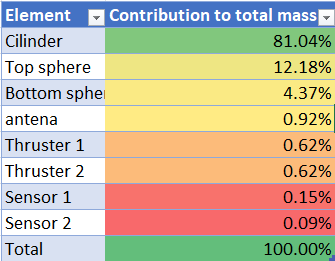
\includegraphics[width=\maxwidth{33.61766181635725em}]{image_1}
\end{center}
\end{par}


\vspace{1em}
\matlabheading{Calculating Inertias}


\vspace{1em}
\matlabheadingtwo{Cylinder and Thrusters}

\begin{par}
$$\mathrm{Ix}=\frac{1}{2}{\mathrm{mr}}^2$$
\end{par}

\begin{par}
$$\textrm{Iy}=\textrm{Iz}=\frac{1}{4}{\textrm{mr}}^2 +\frac{1}{12}{\textrm{mh}}^2$$
\end{par}

\matlabheadingthree{        Cylinder}

\begin{par}
\hfill \break
\end{par}

\begin{matlabcode}
r = 0.115;
h = 1.25;

Ix =  1/2*m_cylinder*r^2;
Iy = 1/4*m_cylinder*r^2 + 1/12*m_cylinder*h^2;
Iz = Iy;


\end{matlabcode}

\begin{par}
\begin{flushleft}
Building the matrix:  
\end{flushleft}
\end{par}

\begin{matlabcode}
mat_cyl = RealMassMatrixbuilder(m_cylinder, Ix, Iy, Iz)
\end{matlabcode}
\begin{matlaboutput}
mat_cyl = 6x6    
   42.1424         0         0         0         0         0
         0   42.1424         0         0         0         0
         0         0   42.1424         0         0         0
         0         0         0    0.2787         0         0
         0         0         0         0    5.6266         0
         0         0         0         0         0    5.6266

\end{matlaboutput}

\begin{par}
\begin{flushleft}
Tranlsating the matrix from element  body center to   SPARUS Grav 
\end{flushleft}
\end{par}

\begin{matlabcode}
trans_cyl = Translation(0.12, 0, 0, mat_cyl)
\end{matlabcode}
\begin{matlaboutput}
trans_cyl = 6x6    
   42.1424         0         0         0         0         0
         0   42.1424         0         0         0    5.0571
         0         0   42.1424         0   -5.0571         0
         0         0         0    0.2787         0         0
         0         0   -5.0571         0    6.2335         0
         0    5.0571         0         0         0    6.2335

\end{matlaboutput}

\matlabheadingthree{        Thruster 1}

\begin{par}
\hfill \break
\end{par}

\begin{matlabcode}
r = 0.035;
h = 0.25;

Ix =  1/2*m_thruster1*r^2;
Iy = 1/4*m_thruster1*r^2 + 1/12*m_thruster1*h^2;
Iz = Iy;

\end{matlabcode}

\begin{par}
\begin{flushleft}
Building the matrix:  
\end{flushleft}
\end{par}

\begin{matlabcode}
mat_thr1 = RealMassMatrixbuilder(m_thruster1, Ix, Iy, Iz)
\end{matlabcode}
\begin{matlaboutput}
mat_thr1 = 6x6    
    0.3220         0         0         0         0         0
         0    0.3220         0         0         0         0
         0         0    0.3220         0         0         0
         0         0         0    0.0002         0         0
         0         0         0         0    0.0018         0
         0         0         0         0         0    0.0018

\end{matlaboutput}

\begin{par}
\begin{flushleft}
Tranlsating the matrix from element  body center to   SPARUS Grav 
\end{flushleft}
\end{par}

\begin{matlabcode}
trans_thr1 = Translation(-0.59, 0.17, 0, mat_thr1)
\end{matlabcode}
\begin{matlaboutput}
trans_thr1 = 6x6    
    0.3220         0         0         0         0   -0.0547
         0    0.3220         0         0         0   -0.1900
         0         0    0.3220    0.0547    0.1900         0
         0         0    0.0547    0.0095    0.0323         0
         0         0    0.1900    0.0323    0.1138         0
   -0.0547   -0.1900         0         0         0    0.1232

\end{matlaboutput}

\matlabheadingthree{        Thruster 2}

\begin{par}
\hfill \break
\end{par}

\begin{matlabcode}
r = 0.035;
h = 0.25;

Ix =  1/2*m_thruster1*r^2;
Iy = 1/4*m_thruster1*r^2 + 1/12*m_thruster1*h^2;
Iz = Iy;
\end{matlabcode}

\begin{par}
\begin{flushleft}
Building the matrix:  
\end{flushleft}
\end{par}

\begin{matlabcode}
mat_thr2 = RealMassMatrixbuilder(m_thurster2, Ix, Iy, Iz)
\end{matlabcode}
\begin{matlaboutput}
mat_thr2 = 6x6    
    0.3220         0         0         0         0         0
         0    0.3220         0         0         0         0
         0         0    0.3220         0         0         0
         0         0         0    0.0002         0         0
         0         0         0         0    0.0018         0
         0         0         0         0         0    0.0018

\end{matlaboutput}

\begin{par}
\begin{flushleft}
Tranlsating the matrix from element  body center to   SPARUS Grav 
\end{flushleft}
\end{par}

\begin{matlabcode}
trans_thr2 = Translation(-0.59, -0.17, 0, mat_thr2)
\end{matlabcode}
\begin{matlaboutput}
trans_thr2 = 6x6    
    0.3220         0         0         0         0    0.0547
         0    0.3220         0         0         0   -0.1900
         0         0    0.3220   -0.0547    0.1900         0
         0         0   -0.0547    0.0095   -0.0323         0
         0         0    0.1900   -0.0323    0.1138         0
    0.0547   -0.1900         0         0         0    0.1232

\end{matlaboutput}

\matlabheadingtwo{Sensors }


\vspace{1em}
\begin{par}
$$\mathrm{Ix}=\mathrm{Iy}=\frac{1}{4}{\mathrm{mr}}^2 +\frac{1}{12}{\mathrm{mh}}^2$$
\end{par}

\begin{par}
$$\textrm{Iz}=\frac{1}{2}{\textrm{mr}}^2$$
\end{par}

\matlabheadingthree{    Sensor 1}

\begin{par}
\hfill \break
\end{par}

\begin{matlabcode}
r = 0.05;
h = 0.03;

Ix =  1/4*m_sensor1*r^2 + 1/12*m_sensor1*h^2;
Iy = Ix;
Iy = 1/2*m_sensor1*r^2;
\end{matlabcode}

\matlabheadingthree{    }

\begin{par}
\begin{flushleft}
Building the matrix:  
\end{flushleft}
\end{par}

\begin{matlabcode}
mat_sens1 = RealMassMatrixbuilder(m_sensor1, Ix, Iy, Iz)
\end{matlabcode}
\begin{matlaboutput}
mat_sens1 = 6x6    
    0.0796         0         0         0         0         0
         0    0.0796         0         0         0         0
         0         0    0.0796         0         0         0
         0         0         0    0.0001         0         0
         0         0         0         0    0.0001         0
         0         0         0         0         0    0.0018

\end{matlaboutput}

\begin{par}
\begin{flushleft}
Tranlsating the matrix from element  body center to   SPARUS Grav 
\end{flushleft}
\end{par}

\begin{matlabcode}
trans_sens1 = Translation(0.7, 0, -0.14, mat_sens1)
\end{matlabcode}
\begin{matlaboutput}
trans_sens1 = 6x6    
    0.0796         0         0         0   -0.0111         0
         0    0.0796         0    0.0111         0    0.0557
         0         0    0.0796         0   -0.0557         0
         0    0.0111         0    0.0016         0    0.0078
   -0.0111         0   -0.0557         0    0.0407         0
         0    0.0557         0    0.0078         0    0.0408

\end{matlaboutput}

\matlabheadingthree{ }

\matlabheadingthree{   Sensor 2}

\begin{par}
\hfill \break
\end{par}

\begin{matlabcode}
r = 0.05;
h = 0.05;

Ix =  1/4*m_sensor2*r^2 + 1/12*m_sensor2*h^2;
Iy = Ix;
Iy = 1/2*m_sensor2*r^2;

\end{matlabcode}

\begin{par}
\begin{flushleft}
Building the matrix:  
\end{flushleft}
\end{par}

\begin{matlabcode}
mat_sens2 = RealMassMatrixbuilder(m_sensor2, Ix, Iy, Iz)
\end{matlabcode}
\begin{matlaboutput}
mat_sens2 = 6x6    
    0.0479         0         0         0         0         0
         0    0.0479         0         0         0         0
         0         0    0.0479         0         0         0
         0         0         0    0.0000         0         0
         0         0         0         0    0.0001         0
         0         0         0         0         0    0.0018

\end{matlaboutput}

\matlabheadingthree{ }

\begin{par}
\begin{flushleft}
Tranlsating the matrix from element  body center to   SPARUS Grav 
\end{flushleft}
\end{par}

\begin{matlabcode}
trans_sens2 = Translation(0.44, 0, -0.14, mat_sens2)
\end{matlabcode}
\begin{matlaboutput}
trans_sens2 = 6x6    
    0.0479         0         0         0   -0.0067         0
         0    0.0479         0    0.0067         0    0.0211
         0         0    0.0479         0   -0.0211         0
         0    0.0067         0    0.0010         0    0.0030
   -0.0067         0   -0.0211         0    0.0103         0
         0    0.0211         0    0.0030         0    0.0111

\end{matlaboutput}

\matlabheadingtwo{Top  and bottom Sphere}

\vspace{1em}

\begin{par}
$$\textrm{Ix}\;=\frac{3}{10}mr^2$$
\end{par}

\begin{par}
$$\textrm{Iy}=\textrm{Iz}\;=m\frac{3}{20}r^2 +m\frac{1}{10}h^2$$
\end{par}

\matlabheadingthree{        Top Shpere}

\begin{par}
\hfill \break
\end{par}

\begin{matlabcode}
r = 0.115;
h = 0.25;

Ix =  3/10*m_topsphere*r^2;
Iy = m_topsphere*(3/20*r^2 + 1/10*h^2);
Iz = Iy;


\end{matlabcode}

\begin{par}
\begin{flushleft}
Building the matrix:  
\end{flushleft}
\end{par}

\begin{matlabcode}
mat_TS = RealMassMatrixbuilder(m_topsphere, Ix, Iy, Iz)
\end{matlabcode}
\begin{matlaboutput}
mat_TS = 6x6    
    6.3335         0         0         0         0         0
         0    6.3335         0         0         0         0
         0         0    6.3335         0         0         0
         0         0         0    0.0251         0         0
         0         0         0         0    0.0521         0
         0         0         0         0         0    0.0521

\end{matlaboutput}

\begin{par}
\begin{flushleft}
Tranlsating the matrix from element  body center to   SPARUS Grav 
\end{flushleft}
\end{par}

\begin{matlabcode}
trans_TS = Translation(0.8, 0, 0, mat_TS)
\end{matlabcode}
\begin{matlaboutput}
trans_TS = 6x6    
    6.3335         0         0         0         0         0
         0    6.3335         0         0         0    5.0668
         0         0    6.3335         0   -5.0668         0
         0         0         0    0.0251         0         0
         0         0   -5.0668         0    4.1056         0
         0    5.0668         0         0         0    4.1056

\end{matlaboutput}

\matlabheadingthree{        Bottom Sphere}

\begin{par}
\hfill \break
\end{par}

\begin{matlabcode}
r = 0.115;
h = 0.25;

Ix = 3/10*m_bottomsphere*r^2;
Iy = m_bottomsphere*(3/20*r^2 + 1/10*h^2);
Iz = Iy;

\end{matlabcode}

\begin{par}
\begin{flushleft}
Building the matrix:  
\end{flushleft}
\end{par}

\begin{matlabcode}
mat_BS = RealMassMatrixbuilder(m_bottomsphere, Ix, Iy, Iz)
\end{matlabcode}
\begin{matlaboutput}
mat_BS = 6x6    
    2.2736         0         0         0         0         0
         0    2.2736         0         0         0         0
         0         0    2.2736         0         0         0
         0         0         0    0.0090         0         0
         0         0         0         0    0.0187         0
         0         0         0         0         0    0.0187

\end{matlaboutput}

\begin{par}
\begin{flushleft}
Tranlsating the matrix from element  body center to   SPARUS Grav 
\end{flushleft}
\end{par}

\begin{matlabcode}
trans_BS = Translation(-0.64, 0, 0, mat_BS)
\end{matlabcode}
\begin{matlaboutput}
trans_BS = 6x6    
    2.2736         0         0         0         0         0
         0    2.2736         0         0         0   -1.4551
         0         0    2.2736         0    1.4551         0
         0         0         0    0.0090         0         0
         0         0    1.4551         0    0.9500         0
         0   -1.4551         0         0         0    0.9500

\end{matlaboutput}

\matlabheadingtwo{Antena }

\begin{par}
$$\textrm{Ix}=\frac{1}{12}m\left(h^2 +d^2 \right)$$
\end{par}

\begin{par}
$$\textrm{Iy}=\frac{1}{12}m\left(h^2 +w^2 \right)$$
\end{par}

\begin{par}
$$\textrm{Iz}=\frac{1}{12}m\left(w^2 +d^2 \right)$$
\end{par}

\begin{matlabcode}
w = 0.05;
d = 0.04;
h = 0.25;


Ix = 1/12*m_antena*(h^2+d^2);
Iy = 1/12*m_antena*(h^2+w^2);
Iz = 1/12*m_antena*(w^2+d^2);
\end{matlabcode}

\begin{par}
\begin{flushleft}
Building the matrix:  
\end{flushleft}
\end{par}

\begin{matlabcode}
mat_ant = RealMassMatrixbuilder(m_antena, Ix, Iy, Iz)
\end{matlabcode}
\begin{matlaboutput}
mat_ant = 6x6    
    0.4791         0         0         0         0         0
         0    0.4791         0         0         0         0
         0         0    0.4791         0         0         0
         0         0         0    0.0026         0         0
         0         0         0         0    0.0026         0
         0         0         0         0         0    0.0002

\end{matlaboutput}

\begin{par}
\begin{flushleft}
Tranlsating the matrix from element  body center to   SPARUS Grav 
\end{flushleft}
\end{par}

\begin{matlabcode}
trans_ant = Translation(-0.4, 0, -0.25, mat_ant)
\end{matlabcode}
\begin{matlaboutput}
trans_ant = 6x6    
    0.4791         0         0         0   -0.1198         0
         0    0.4791         0    0.1198         0   -0.1916
         0         0    0.4791         0    0.1916         0
         0    0.1198         0    0.0325         0   -0.0479
   -0.1198         0    0.1916         0    0.1092         0
         0   -0.1916         0   -0.0479         0    0.0768

\end{matlaboutput}

\vspace{1em}

\matlabheading{Calculating the Total Mass Marix}

\begin{matlabcode}
Real_Mass = trans_ant + trans_BS + trans_TS + trans_sens2 + trans_sens1 + trans_thr2 + trans_thr1 + trans_cyl
\end{matlabcode}
\begin{matlaboutput}
Real_Mass = 6x6    
   52.0000         0         0         0   -0.1376         0
         0   52.0000         0    0.1376         0    8.1741
         0         0   52.0000         0   -8.1741         0
         0    0.1376         0    0.3669         0   -0.0372
   -0.1376         0   -8.1741         0   11.6769         0
         0    8.1741         0   -0.0372         0   11.6640

\end{matlaboutput}

\begin{par}
\begin{flushleft}
 
\end{flushleft}
\end{par}

\end{document}
